\section{Sistema de observaciones}

Como ya habiamos explicado anteriormente, para obtener las observaciones necesitabamos capturar las imagenes producidas por el juego y enviarlas a los agentes para que entrenaran. La principal dificultad es que el juego y el entorno de Python son procesos completamente distintos asi que era necesario crear una forma de compartir esta infomacion.

Planteamos dos alternativas para resolver el problema:

\subsection*{Alternativa 1: Sockets}

La primera alternativa consistia en que al comenzar el juego, conseguir que todo el output visual fuera enviado a traves de un socket que estaría conectado con el proceso de Python. Para implementar esta comunicacion con sockets, ambos procesos deberian crear un thread encargado de la comunicacion, ademas del thread principal. En la figura \ref {fig:alternativa-1-com} podemos ver un esquema de la arquitectura de esta alternativa.

\begin{figure}[ht]
    \centering
    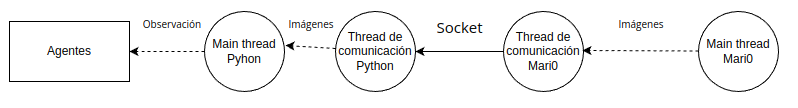
\includegraphics[width=1.0\textwidth]{img/Observations-1.png}
    \caption{Esquema de la alternativa por sockets[Elaboración Propia]}
    \label{fig:alternativa-1-com}
\end{figure}

Esta alternativa tiene diferentes problemas. El problema principal es que realizar el envio de las imagenes a traves de sockets es un proceso complejo y de programación de bajo nivel. Esto requeriría coordinación entre procesos, decidir cuantas capturas de pantalla se enviarán por segundo para no saturar el canal de comunicación, comunicar los thread de Python, modificar casi por completo el renderizado del videojuego, etc.

\subsection*{Alternativa 2: Virtual frame buffer}

La segunda alternativa es usar un Virtual frame buffer para capturar las imagenes del videojuego y luego usar la libreria mss \cite {mss} para tomar capturas de este buffer. Esta alternativa es usada en otros proyectos de OpenAI similares como \cite {muphen}. En primer lugar explicaremos que es un Virtual frame buffer.

Un Virtual frame buffer (Xvfb) es un servidor de sistema de ventanas que ejecuta todas las operaciones graficas en memoria sin mostrar nada por pantalla \cite {xvfb-wikipedia}. De forma simple, es un proceso que actua como una pantalla virtual donde pueden realizarse tareas graficas como abrir un navegador, jugar a un videojuego, etc. pero sin mostrar ninguna imagen por la pantalla real, todo ocurre en la memoria del ordenador.

El modulo mss es simplemente una libreria capaz de tomar capturas de pantalla eficientemente de cualquier display, ya sea un display virtual como en nuestro caso o de la pantalla del ordenador.

Usando esta tecnologia, deberiamos seguir el siguiente proceso. El proceso de Python debería crear el proceso de Xvfb y mas tarde el proceso de Mari0, que usará el Xvfb para renderizar el juego. Finalmente, cuando sea necesario obtener una observacion del entorno, el modulo mss se encargará de obtener una captura de pantalla de Xvfb. Podemos ver el esquema de esta alternativa en la figura \ref{fig:alternativa-2-com}. En la figura \ref {fig:alternativa-2-seq} podemos ver el diagrama de secuencia de esta alternativa.

\begin{figure}[ht]
    \centering
    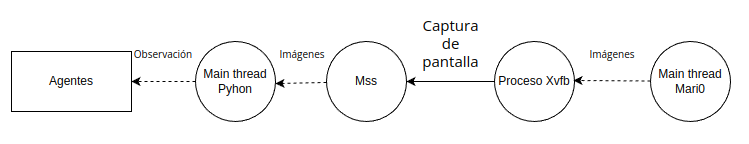
\includegraphics[width=1.0\textwidth]{img/Obsertavions-2.png}
    \caption{Esquema de la alternativa por Xvfb [Elaboración Propia]}
    \label{fig:alternativa-2-com}
\end{figure}

\begin{figure}[ht]
    \centering
    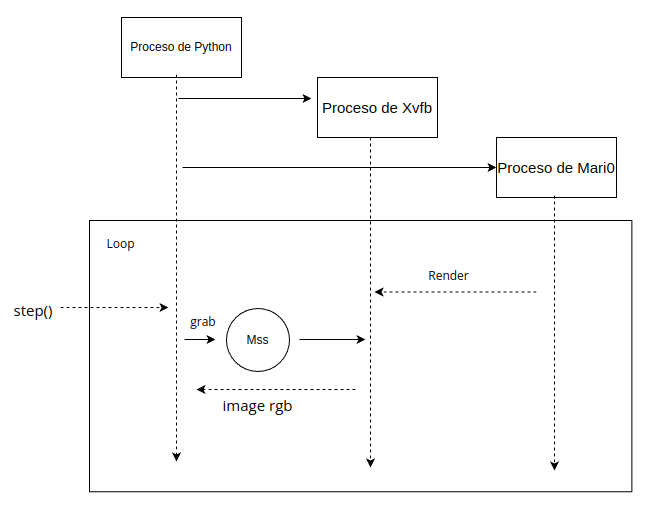
\includegraphics[width=1.0\textwidth]{img/obsevation_sequence.png}
    \caption{Diagrama de secuencia de la alternativa por Xvfb [Elaboración Propia]}
    \label{fig:alternativa-2-seq}
\end{figure}

Esta alternativa es mucho más simple que la alternativa por sockets, ademas, no requiere modificar el sistema de renderizado del videojuego ni tampoco sincronización de threads ni comunicación entre sockets. 

Otra ventaja de esta alternativa es que nos permite observar el funcionamiento del entorno desde 0 e incluso interactuar directamente con el entorno grafico usando un servidor y cliente de VNC. Esto es muy util para visualizar el entorno y sobretodo para la fase de testing. Cubriremos este proceso en la fase de testing.

Finalmente, implementar la función render de PettingZoo sería aparentemente sencillo, ya que solo deberiamos usar captura de pantalla del modulo mss en el modulo pygame.

Por estos motivos, para el sistema de observaciones escogimos la alternativa por Xvfb. Aún así, la idea basica de la alternativa 1 sería usada para el sistema de comunicacion entre procesos, que explicaremos más adelante. 

Además de todo lo explicado anteriormente, tambien implementamos la posibilidad de que un humano pudiera jugar al mismo tiempo que una IA. Para poder lograr esto desactivamos el uso del virtual frame buffer, así el humano podría ver la escena en su monitor. Sin embargo, hay dos pequeñas desventaja, el usuario que vaya a jugar deberá calcular la posición de la ventana del juego en su monitor y este tambien podría controlar el movimiento de los agentes si quisiera. El primer problema se debe a que no es posible saber la posición de la pantalla desde el programa de Python. Y el segundo se debe a que el usuario podría usar las teclas asignadas al movimiento de otros jugadores y así controlar el movimiento del jugador asignado a la IA.


\subsubsection*{Problemas encontrados}

Realizando la implementación de las observaciones nos encontramos con varios problemas. En esta seccion explicaremos brevemente los problemas que tuvimos y su solucion.

\begin{itemize}
    \item Conseguir que el proceso de Mari0 usase el virtual frame buffer en vez de la pantalla. Para esto, es necesario cambiar la variable de entorno del sistema 'display'. Una vez cambiada y creado el proceso es necesario resetearla de fabrica puesto que podría ocasionar problemas al iniciar otros procesos.
    \item Conseguir que el modulo de pygame renderizara el contenido de la captura de pantalla. Para conseguir esto tuvimos que adaptar el contenido de la screenshot, que venía en formato BRGA a formator RGB.
    \item Si el programa de Python se cierra de forma abrupta, es posible que el proceso de Mari0 y de Xvfb queden zombies en el sistema. Este problema no se pudo solucionar directamente puesto que no podemos controlar cuando el programa se abortará. La unica solución es acabar el programa manualmente usando la consola de Linux.
\end{itemize}



